\documentclass[12pt]{article}

% set margins and spacing
\addtolength{\textwidth}{1.3in}
\addtolength{\oddsidemargin}{-.65in} %left margin
\addtolength{\evensidemargin}{-.65in}
\setlength{\textheight}{9in}
\setlength{\topmargin}{-.5in}
\setlength{\headheight}{0.0in}
\setlength{\footskip}{.375in}
\renewcommand{\baselinestretch}{1.0}
\linespread{1.0}

% load miscellaneous packages
\usepackage{csquotes}
\usepackage[american]{babel}
\usepackage[usenames,dvipsnames]{color}
\usepackage{graphicx,amsbsy,amssymb, amsmath, amsthm, MnSymbol,bbding,times, verbatim,bm,pifont,pdfsync,setspace,natbib}
\usepackage{wrapfig}
\usepackage{multirow, amsmath}
\usepackage{ulem}
\usepackage[table]{xcolor}
\usepackage{booktabs} 



% enable hyperlinks and table of contents
\usepackage[pdftex,
bookmarks=true,
bookmarksnumbered=false,
pdfview=fitH,
bookmarksopen=true,hyperfootnotes=false]{hyperref}
\hypersetup{colorlinks=true, linkcolor=blue, citecolor=blue}

% enable flowchart diagram package
\usepackage{tikz}
\usetikzlibrary{shapes.geometric, arrows}
\usepackage{graphicx}

% define environments
\newtheorem{definition}{Definition}
\newtheorem{fact}{Fact}
\newtheorem{result}{Result}
\newtheorem{proposition}{Proposition}



\begin{document}
\title{Crime and Drug Treatment across Detroit}
\author{Rachel Gaudreau\thanks{Syracuse University, Economics Department. Email: regaudre@syr.edu.} \and Sophia Oritz-Heaney\thanks{Syracuse University, Economics Department. Email: sgortizh@syr.edu} \and Weston Maechling\thanks{Syracuse University, Economics Department. Email: wrmaechl@syr.edu.} \and Leo Gershman\thanks{Syracuse University, Economics Department. Email: lgershman@syr.edu}}
\date{\vskip-.1in \today}
\maketitle

\bigskip
\begin{center} {\bf Abstract} \end{center}

\begin{quote}
    {\small In this study, we study the relationship between the distance from a substance abuse treatment center (SATC) and the number of 911 calls in the Greater Detroit area. This paper creates a framework that locates the SATCs in the Greater Detroit area and then creates rings around them at distances ranging from 50 to 2500 meters to find the number of calls within each ring. Our analysis gathers all the calls to the Detroit Police Department in 2017. Using this data, we conduct an array of t-tests to test if there is a lower likelihood of calls the further someone is from a SATC. With the help of the "City of Detroit's Open Data Portal," we can obtain information on the type of call along with precisely when and where it occurred. This paper finds the number of calls between the distance to an SATC and a 911 call. A t-test is conducted with this information to find the difference in 911 calls per ring around an SATC. We did this for all 911 calls and for calls that involved crimes. The results show that the more 911 calls and crimes reported, the closer it is to an SATC. There are various potential reasons behind this reaction, many of which this paper explores further. The potential importance of this paper comes from the relationship between 911 calls and SATCs, which could help infrastructure planning in similar urban areas.} 
\end{quote}

\bigskip
\section{Introduction} \label{sec:introduction}
A common concern among the general public in the United States is the increase in crime rates. According to \cite{covid_and_crime}, this number is more than fifty percent. In addition, drug usage is another public concern for the American public, especially in urban centers. This paper seeks to determine how the number of 911 calls increases or falls based on the distance to an SATC. Our hypothesis states that closer proximity to SATCs increases access to drug rehabilitation and mental health resources, which, in turn, decreases drug use. This reduction in drug usage would theoretically lead to a decrease in drug-related crimes and, consequently, fewer calls to 911. In what follows, we explore the question, "How does the distance to the closest drug rehabilitation center relate to the number of calls to 911?" 

Our hypothesis is based on the established impact of drug rehabilitation centers on community well-being. \cite{SAT_centers_and_crime} shows that the recent opening of an SATC is correlated with a decrease in all violent crimes and drug use. Studies such as \cite{drugs_and_crime}
and \cite{drugs_crime_space_time} have shown that these centers can lower crime rates and raise living standards in surrounding areas. Thus, SATCs can help the well-being of the community by doing more than preventing crime. \cite{mental_healthcare_and_crime}, an article showing that drug dependency is one of the leading causes of criminal behavior, agrees with this by showing that communities prosper through preventive measures. By reducing this dependency, SATCs improve crime rates in their neighborhoods. The lack of criminal behavior allows people to fully embrace better lives closer to their communities fully, decreasing the number of 911 calls. 

To explore the relationship between crime and SATC, we conducted a spatial analysis of Wayne County, Michigan. We mapped the locations of drug rehabilitation centers along with the 911 calls. Our results show that areas closer to SATCs had a higher number of 911 calls per square meter when compared to areas further away. Interestingly, further analysis revealed that this trend persisted even when isolating calls related to criminal activities. This data does not support our hypothesis. Nonetheless, as argued in \cite{Socioeconomic-Determinants}, a higher amount of drug usage in an area causes an increase in drug usage. Instead, we find that more 911 calls, and thus drug usage, are closer to SATCs instead of further away from them, as previously argued. 

A potential explanation for these findings could be the reluctance of wealthier communities to permit SATCs to build in their neighborhoods. They could fear that such facilities might attract individuals they perceive as a threat due to their unstable nature as addicts, as shown in \cite{mental_health_and_disability}. It is also possible that these locations are selected to be where they could have the most immediate impact. These are places that have the highest rates of crime and drug usage. It can be hypothesized that it would be worse without a nearby SATC. Most SATCs in Wayne County have been constructed within the last decade. These issues do not go away immediately. From that point of view, it is entirely logical that the SATCs would be near the places with the highest drug-related crime.

Answering this question is crucial for developing strategies to mitigate drug-related crimes along with crimes as a whole in American cities. As shown in \cite{SAT_centers_and_crime}, drugs are a significant source of civil unrest, social discord, and crime, particularly in urban areas. This is especially true in historically unsupported areas by government resources. By understanding the relationship between SATC location and emergency call frequency, we can work toward solutions that foster safer and healthier communities. Our paper attempts to provide further insight into the relationship between SATCs and crime in Detroit. In doing so, we hope to further knowledge about the field of social economics and the consequences of SATC presence in an area. However, the paper can be improved by adding more cities, seeing the relationship between the amount of 911 calls over the years, or finding a control for the nominal SATC and what would happen to a community without them. Our study shows how SATCs commonly find themselves in areas with higher rates of 911 calls. We further build off that by extrapolating on why that could be the case and what it means for the future of Wayne County.



\section{Literature Review} \label{sec:literature}
The geographical relationship between crime and access to mental health care is a widely studied topic. The results can seem conflicting based on the factors considered in the research.  For example, mental illness is associated with an increased likelihood of substance abuse, which directly and indirectly relates an increase in crime. One viable method of treating mental illness is through office-based mental healthcare. Evidence shows that increasing access to office-based mental health care by 10 mental health care provider offices in a county can lead to a 0.4\% reduction in the county crime rate (\cite{mental_healthcare_and_crime}). An increase in access to mental health care also shows a connection to participation in government disability programs. Furthermore, this effect is also evident when specifically considering access to SATC facilities. Evidence shows that increasing access to SAT facilities reduces violent crime due to the effectiveness in reducing crimes motivated by obtaining money to purchase drugs, reducing violence among those in the drug trade, and reducing drug usage which eases aggressive behavior due to drug abuse (\cite{SAT_centers_and_crime}). 

However, a significant barrier to treatment could be the price of substance abuse treatment. In a study conducted between 2002 and 2003, the median willingness to pay for drug rehabilitation is shown to be below the average cost of treatment. Moreover, the cost of drug treatment is a significant indicator of self-reported probability of enrollment (\cite{cost_of_drug_treatment}). While it is likely that cost of treatment has changed in the subsequent decades, it is still important to acknowledge barriers to treatment when considering its affects on crime rates in an urban area, such as Detroit. 

Barriers to  treatment also contribute to evidence of a positive feedback loop between drug usage, crime, and standard of living in a given area. The drug trade, specifically the sale and use of drugs in a given area has been closely linked to an increase in the crime rate in the vicinity. A case study of Miami-Dade county shows that drug activity on a given block can alter or nullify the relationship between household income and crime. Thus, drug usage can be a predictor of crime rates in a geographical area (\cite{drugs_crime_space_time}). This effect also has implications on an area's living standards. Since higher levels of drug usage leads to higher crime rates in a given geographical area, this corresponds to lower standards of living. This effect is due to the addictive properties of drugs, the poor decision making caused by drug usage, and the relationship between areas with lower standards of living and a higher tendency for those who live in those areas to turn to drugs as a means for escape (\cite{drugs_and_crime}).

Moreover, given our focus on crime it is important to understand the impact the COVID-19 Pandemic had on crime in general. Practices such as social distancing and at-home quarantines led people to spend more time in privately occupied spaces. This led to a decrease in the amount of crimes committed in a public setting, such as robbery, homicide, physical violence, etc. However, this also led to an increase in crimes committed in private settings, such as domestic violence \cite{covid_and_crime}. Since COVID-19 had a varied affect on crime for the purposes of our analysis we decided to limit our study of crime prior to the COVID-19 Pandemic.

Considering the conflicting theories on how drugs, crime, and drug treatment are related and the effects on a geographical area, we show how a SATC affects the number of 911 calls in an area which represent the perceived crime and, conversely, safety of an area. Understanding this effect will give insight into possible policies to reduce crime in an area. Furthermore, given the lack of economic research on this topic we decided to focus on a single case study, in this instance, Detroit, and the immediate surrounding communities to analyze the effects a SATC has on crime in its surrounding area. 

\section{Theoretical Analysis}
\label{sec:theory}
This paper assesses the hypothesis that the number of 911 calls increases as a person moves further away from an SATC. \cite{SAT_centers_and_crime} demonstrates how the crime rate is negatively related to the number of SATCs. As more centers open, they can provide treatment to people who previously could not receive any due to distance constraints. A decrease in dependency on emergency services was also found in conjunction with crime. The decrease in dependence on all forms of emergency services follows along with what \cite{Socioeconomic-Determinants} found: lower drug usage in an area causes the people who live there to have more stable and prosperous lives. It shows that as someone frees themselves from drug addiction and increases their socioeconomic standing, they become more productive members of society. This greater access to treatment caused overall crime rates to drop as there was a reduction in crimes motivated by drugs or getting the money to acquire more. We can connect it with the findings of \cite{drugs_and_crime}, who found that a decrease in drug use for an area positively correlates with the change in crime in the same area. This rise in both drug usage and crime causes a negatively related change in the standards of living of that area, which they found will again negatively relate to the amount of drug usage restarting the cycle. This framework allowed us to analyze our claim (see Figure 1) that the distance to the closest SATC will impact the ability to receive treatment, which will decrease the level of drug use in that area, leading to a positively related effect on drug-related crimes and also positively affecting the total number of 911.



\section{Data}
\label{sec:data}

\subsection{911 Calls in Detroit Area}

This data comes from the City of Detroit Open Data Portal's   \href{https://data.detroitmi.gov/datasets/detroitmi::police-serviced-911-calls/about}{Police Serviced 911 Calls}. It is generated by the Detroit Police Department's Crime Data Analytics when a call is placed. This data set covers 911 calls that are received by precincts around the Detroit metropolitan area from the year 2016-2022. There are 5,238,111 observations. Key variables include incident year, latitude, longitude, call category and call description. The longitude and latitude coordinates of all 911 calls in this dataset are geo-coded in the left graph in Figure~\ref{fig:Figure2}. They are color-coded blue. 

We isolated our data from both Police Serviced 911 Calls and N-SSATS to one year, 2017, from the original dataset so we could perform cross-sectional analysis. There are 620,359 observations in 2017 alone. We chose observations from 2017 since the year a) overlaps with the second set of data and b) is before COVID-19, where crime rate statistics shifted in general \cite{covid_and_crime}. This is to eliminate COVID-19 effects from affecting our data analysis. Years 2016, 2018, and 2019 could also work for cross-sectional analysis, but for simplicity, we only analyze one year in this report. Cross-sectional analysis should be applied to more years in the future. The data includes latitude and longitude variables, which we used to geocode each call to a single point in space. The longitude and latitudes of just 911 calls in 2017 are geo-coded in the left graph in Figure~\ref{fig:Figure2}. They are color-coded green. 

Additionally, we isolated the 2017 call data only to include calls related to crime. We used the variable call description to identify what calls could be considered to relate to crime. There are 466,219 observations. Our group created this dataset that only involved crimes to focus on activities that drugs could cause. The 9-1-1 emergency telephone hotline is used for more than just crimes; it is used for any civil issue classified as an emergency. By focusing only on the crimes in question, we narrow down the issues to better estimate the impact of SATCs in an area. We theorized that if all calls to emergency services were considered, the results could be diluted by prioritizing areas with higher population densities. These people are not counted because they are unnaffected by a SATC.

\subsection{Substance Abuse Treatment Centers (SATCs) in Detroit Area (Dataset 2)}

This data is from the Substance Abuse and Mental Health Services Administration (SAMHSA). Data is generated through the National Survey of Substance Abuse Treatment Services \href{https://www.samhsa.gov/data/data-we-collect/n-ssats-national-survey-substance-abuse-treatment-services}{N-SSATS}, an annual survey of all known public and private substance abuse treatment services in the United States. SAMHSA conducts this survey annually.  This data covers the names and addresses of substance abuse treatment services in operation in the Detroit Metropolitan area between the years 2015 to 2021. Key variables include year, longitude, latitude, zip code, and services provided listed in priority order. There are 55 variables and 333 observations.\footnotemark[1]\footnotetext[1]{Future research may use variables such as primary service offered to explore how primary treatments offered may affect crime rates. Additionally, since there are only 115 distinct name (SATC) variables in the dataset, future research can explore how the opening or closing of a SATC affects local crime rates.}Although there are 333 observations, there are only 115 distinct SATC names. This means that some SATC overlap between years, while others are only opened and registered for one year within this dataset. 



\subsection{Measuring Distance of each 911 Call to each SATC}
 


\begin{wrapfigure}[14]{r}{0.3\textwidth} 
 \begin{tikzpicture}
% Define the radii corresponding to the first 3 distances (in meters)

\centering
\def\radiusOne{0.5}
\def\radiusTwo{1}
\def\radiusThree{1.75}


% Draw the concentric circles
\foreach \r/\label in {\radiusOne/, 
    \radiusTwo/,
    \radiusThree/,}
 {
\draw[thick] (0,0) circle (\r);
    \node at (\r, 0) {\label};
    }   
    \fill (0,0) circle (2pt);
    \label{fig:Figure1}
\end{tikzpicture}
\caption{Concentric Distance Rings}
\small\textit{Notes: The figure represents the first three distance rings (100m, 250m, 500m). Center dot marks the SATC.}
\end{wrapfigure}

We used layered data sets and geocoded their locations. Using the coordinates (longitude and latitude variables) of each point, we created two new variables. Every 911 call is assigned one SATC, the one geographically closest to it. This will prevent overlap from calls that are within range of multiple treatment centers.

We create distance rings, referred to as distance groups, and perform our analysis. We normalize the data to account for differences in total area of a distance group that may alter results. We did this by dividing the area in squared meters by the total count of 911 calls in each distance group.

We created concentric rings around each SATC. Each 911 point falls within one circle, referred to as a distance ring or distance group, and is counted towards the SATC in its circle's center. Our data is organized by SATC. There are 620,359 observations in total, but only 415,216 observations fall within the geo-coded parameters. Thus, we only analyze the 415,216 calls in relation to SATC proximity. 
\begin{table}[h]
\centering
\scalebox{0.8}{
\centering

\begin{tabular}{l*{6}{c}}
\hline\hline
            &summary\_results&            &            &            &            &            \\
            &         Obs&        Mean&   Std. dev.&         Sum&         Min&         Max\\
\hline
100m        &          44&    2838.745&    3046.525&    124904.8&           0&    11968.45\\
250m        &          44&    1870.036&    1906.982&    82281.59&           0&    8694.407\\
500m        &          44&    1680.406&    1721.943&    73937.87&           0&    7086.002\\
750m        &          44&    1069.475&    711.9805&     47056.9&           0&    2694.175\\
1000m       &          44&    979.8653&    686.1379&    43114.07&           0&     2722.55\\
1250m       &          44&    823.8632&    680.5173&    36249.98&           0&    3141.789\\
1500m       &          44&    563.8347&    565.9372&    24808.73&           0&    2321.463\\
1750m       &          44&    412.9926&    432.5729&    18171.67&           0&    1617.602\\
2000m       &          44&    248.2508&    279.9933&    10923.04&           0&     956.118\\
2250m       &          44&    206.0333&    270.5081&    9065.466&           0&     1019.79\\
2500m       &          44&    135.5787&    178.7922&    5965.462&           0&    655.3833\\
\hline\hline
\end{tabular}


}


\caption{\textbf{All 2017 Calls T-Tests}}
\label{tabl:Table}
\centering\textit{Two sample t-tests of the difference in mean calls per SATC per distance group.}
\textit{Distances in kilometers squared.}
\end{table}


\begin{figure}[h!]
    \centering
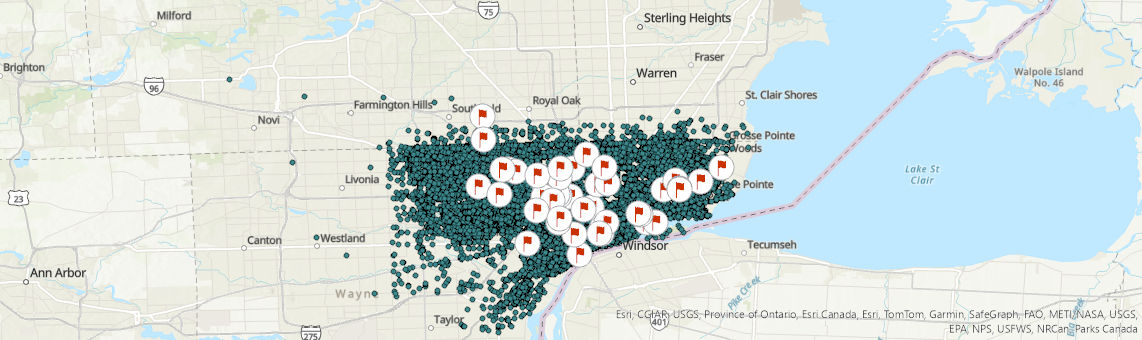
\includegraphics[width=0.75\linewidth]{Reproducibility Package/Visual Graphics/ArcGIS_Map.jpg}
    \caption{Calls and Centers Plotted by Long/Lat}
    \label{fig:Figure2}
     \textit{This visual shows how each call and center data point look when plotted by longitude and latitude.}
     \textit{Each green dot is a call and each red flag is a SATC.}
    
\end{figure}


%Describe your data. Where you got it from, how it was generated, what variables you'll use, what data cleaning steps you had to take, where your processed data, code and documentation is stored.
%In a published paper, a lot of this detail will be in a data appendix. For the purposes of this report, include it all here (this may be the longest section of your report).

\section{Results}
\label{sec:result}

This paper hypothesizes that as the distance from a SATC facility increases, the number of 911 calls also increases. This means that the farther someone is from a SATC, the less access they have to treat drug addiction, so the more likely they would exhibit drug-induced behavior that results in someone calling 911. Our null hypothesis is that there is no relation between distance to an SATC and the likelihood of calling 911. We test the null hypothesis at 90\% confidence interval. 

Our group conducts two sequential pairwise t-tests to examine the statistical likelihood that one distance ring has a greater mean number of calls per SATC than the next larger ring. The first pairwise comparison table is seen in Table~\ref{tabl:Table1}. This two-sample t-test examines the mean calls per SATC between each distance adjacent distance group for all 2017 calls. Our significance level is 0.10.

\begin{table}[htbp]
\begin{center}

\centering
\begin{tabular}{lllll}
\cline{1-5}
\multicolumn{1}{c}{} &
  \multicolumn{1}{|r}{Mean\_1} &
  \multicolumn{1}{r}{Mean\_2} &
  \multicolumn{1}{r}{Difference} &
  \multicolumn{1}{r}{p\_value} \\
\cline{1-5}
\multicolumn{1}{l}{100m-250m} &
  \multicolumn{1}{|r}{2838.745} &
  \multicolumn{1}{r}{1870.036} &
  \multicolumn{1}{r}{968.709} &
  \multicolumn{1}{r}{0.056} \\
\multicolumn{1}{l}{250m-500m} &
  \multicolumn{1}{|r}{1870.036} &
  \multicolumn{1}{r}{1680.406} &
  \multicolumn{1}{r}{189.630} &
  \multicolumn{1}{r}{0.491} \\
\multicolumn{1}{l}{500m-750m} &
  \multicolumn{1}{|r}{1680.406} &
  \multicolumn{1}{r}{1069.475} &
  \multicolumn{1}{r}{610.931} &
  \multicolumn{1}{r}{0.007} \\
\multicolumn{1}{l}{750m-1000m} &
  \multicolumn{1}{|r}{1069.475} &
  \multicolumn{1}{r}{979.865} &
  \multicolumn{1}{r}{89.610} &
  \multicolumn{1}{r}{0.392} \\
\multicolumn{1}{l}{1000m-1250m} &
  \multicolumn{1}{|r}{979.865} &
  \multicolumn{1}{r}{823.863} &
  \multicolumn{1}{r}{156.002} &
  \multicolumn{1}{r}{0.006} \\
\multicolumn{1}{l}{1250m-1500m} &
  \multicolumn{1}{|r}{823.863} &
  \multicolumn{1}{r}{563.835} &
  \multicolumn{1}{r}{260.028} &
  \multicolumn{1}{r}{0.000} \\
\multicolumn{1}{l}{1500m-1750m} &
  \multicolumn{1}{|r}{563.835} &
  \multicolumn{1}{r}{412.993} &
  \multicolumn{1}{r}{150.842} &
  \multicolumn{1}{r}{0.040} \\
\multicolumn{1}{l}{1750m-2000m} &
  \multicolumn{1}{|r}{412.993} &
  \multicolumn{1}{r}{248.251} &
  \multicolumn{1}{r}{164.742} &
  \multicolumn{1}{r}{0.001} \\
\multicolumn{1}{l}{2000m-2250m} &
  \multicolumn{1}{|r}{248.251} &
  \multicolumn{1}{r}{206.033} &
  \multicolumn{1}{r}{42.218} &
  \multicolumn{1}{r}{0.039} \\
\multicolumn{1}{l}{2250m-2500m} &
  \multicolumn{1}{|r}{206.033} &
  \multicolumn{1}{r}{135.579} &
  \multicolumn{1}{r}{70.455} &
  \multicolumn{1}{r}{0.004} \\
\cline{1-5}
\end{tabular}


\end{center}

\caption{\textbf{All 2017 Calls T-Tests}}
\label{tabl:Table1}
\centering\textit{Two sample t-tests of the difference in mean calls per SATC per distance group.}
\textit{Distances in kilometers squared.}
\end{table}


The results of the majority of t-tests in Table~\ref{tabl:Table1} support the rejection of the null hypothesis for eight of the two-sampled t-tests. Five of the pair t-tests exhibit a p-value less than 0.01, indicating statistical significance between sequential distance rings. In addition, two of the tests show p-values less than 0.05, and one test presents a p-value less than 0.10. These are still statistically significant, although less strong than the groups mentioned above. 

For two of the two-sample t-tests, we cannot reject the null hypothesis as the null hypothesis value falls within the 90\% confidence interval. The 250-500 meter and 750-1000 meter ring tests exhibit p-values of 0.491 and 0.392, respectively. These high p-values show no evidence of statistical significance in the mean values of the distance rings. These results could be due to smaller mean differences, as seen in the column "Difference". T-tests that have larger difference values tend to have a smaller p-value. Smaller difference values might mean that the data doesn't vary enough to make a meaningful difference. Having larger data samples might smooth out this issue. However, the lack of significance found could be caused by the range of distance parameters chosen. A change of distance of 250 meters might not be enough of a geospatial distance to properly isolate and identify distance trends around the SATC.

Our group conducts the second sequential pairwise t-test with the crime-only 911 call means per SATC. The pairwise comparison table is seen in Table~\ref{tabl:Table2}. Results are tested at a significance level of 0.10. 


\begin{table}[hb!]
\begin{center}


\centering
\begin{tabular}{lllll}
\cline{1-5}
\multicolumn{1}{c}{} &
  \multicolumn{1}{|r}{Mean\_1} &
  \multicolumn{1}{r}{Mean\_2} &
  \multicolumn{1}{r}{Difference} &
  \multicolumn{1}{r}{p\_value} \\
\cline{1-5}
\multicolumn{1}{l}{100m-250m} &
  \multicolumn{1}{|r}{2182.593} &
  \multicolumn{1}{r}{1398.221} &
  \multicolumn{1}{r}{784.372} &
  \multicolumn{1}{r}{0.041} \\
\multicolumn{1}{l}{250m-500m} &
  \multicolumn{1}{|r}{1398.221} &
  \multicolumn{1}{r}{1328.915} &
  \multicolumn{1}{r}{69.306} &
  \multicolumn{1}{r}{0.754} \\
\multicolumn{1}{l}{500m-750m} &
  \multicolumn{1}{|r}{1328.915} &
  \multicolumn{1}{r}{813.577} &
  \multicolumn{1}{r}{515.338} &
  \multicolumn{1}{r}{0.005} \\
\multicolumn{1}{l}{750m-1000m} &
  \multicolumn{1}{|r}{813.577} &
  \multicolumn{1}{r}{746.648} &
  \multicolumn{1}{r}{66.929} &
  \multicolumn{1}{r}{0.394} \\
\multicolumn{1}{l}{1000m-1250m} &
  \multicolumn{1}{|r}{746.648} &
  \multicolumn{1}{r}{623.514} &
  \multicolumn{1}{r}{123.133} &
  \multicolumn{1}{r}{0.010} \\
\multicolumn{1}{l}{1250m-1500m} &
  \multicolumn{1}{|r}{623.514} &
  \multicolumn{1}{r}{402.102} &
  \multicolumn{1}{r}{221.413} &
  \multicolumn{1}{r}{0.000} \\
\multicolumn{1}{l}{1500m-1750m} &
  \multicolumn{1}{|r}{402.102} &
  \multicolumn{1}{r}{319.975} &
  \multicolumn{1}{r}{82.127} &
  \multicolumn{1}{r}{0.081} \\
\multicolumn{1}{l}{1750m-2000m} &
  \multicolumn{1}{|r}{319.975} &
  \multicolumn{1}{r}{188.563} &
  \multicolumn{1}{r}{131.412} &
  \multicolumn{1}{r}{0.000} \\
\multicolumn{1}{l}{2000m-2250m} &
  \multicolumn{1}{|r}{188.563} &
  \multicolumn{1}{r}{159.420} &
  \multicolumn{1}{r}{29.142} &
  \multicolumn{1}{r}{0.099} \\
\multicolumn{1}{l}{2250m-2500m} &
  \multicolumn{1}{|r}{159.420} &
  \multicolumn{1}{r}{104.491} &
  \multicolumn{1}{r}{54.930} &
  \multicolumn{1}{r}{0.005} \\
\cline{1-5}
\end{tabular}



\end{center}


\caption{\bf{2017 Crime Calls Two Sample T-Tests}}
\label{tabl:Table2}
\centering\textit{Two sample t-tests of the difference in mean crime only calls per SATC per distance group.}
\textit{Distances in kilometers squared.}
\end{table}


The results of the majority of t-tests in Table~\ref{tabl:Table2} support the rejection of the null hypothesis for eight of the two-sample t-tests. Four of the tests reveal p-values equal to or less than 0.01, two of the tests show p-values less than or equal to 0.05, and two of the t-tests present p-values less than 0.10. 

There are two two-sample t-tests where the p-values are not statistically significant, and, therefore, we can not reject the null hypothesis. The 250-500 meter t-test and the 750-1000 meter t-tests have p-values of 0.754 and 0.394, respectively. These do not fall within the 0.10 significance level. These t-tests are the same distance groups as the t-tests in Table~\ref{tabl:Table1} that were also not statistically significant. This reflects a pattern in the mean call data per SATC for these distance groups. The same reasons as above might apply here.

With the exception of the 100-250 meter group (p-value change from 0.056 to 0.041.), almost every p-value in Table~\ref{tabl:Table2} is larger than the same distance group's p-value in Table~\ref{tabl:Table1}. This could be due to fewer observations in the dataset, decreasing the confidence in the significant meaning of a difference in average calls. 

\begin{figure}[htbp]
    \centering
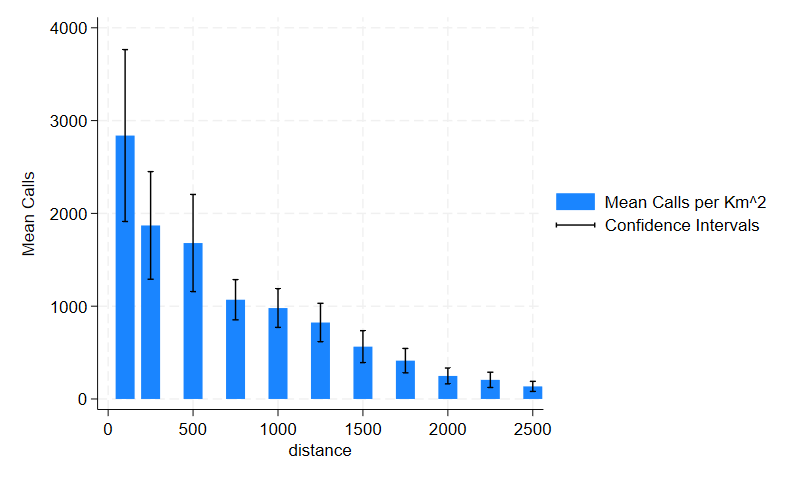
\includegraphics[width=0.75\linewidth]{Reproducibility Package/Visual Graphics/CI_Graph.png}
    \caption{Mean Calls per SATC per distance group}
    \label{fig:Figure3}
     \textit{X-axis consist of the different distance groups used. Distance measured in meters.}
    \textit{Y-axis is measured in mean calls per kilometers squared.}
    \textit{Confidence thresholds measured at 90\%.}
\end{figure}

\begin{figure}[htbp]
    \centering
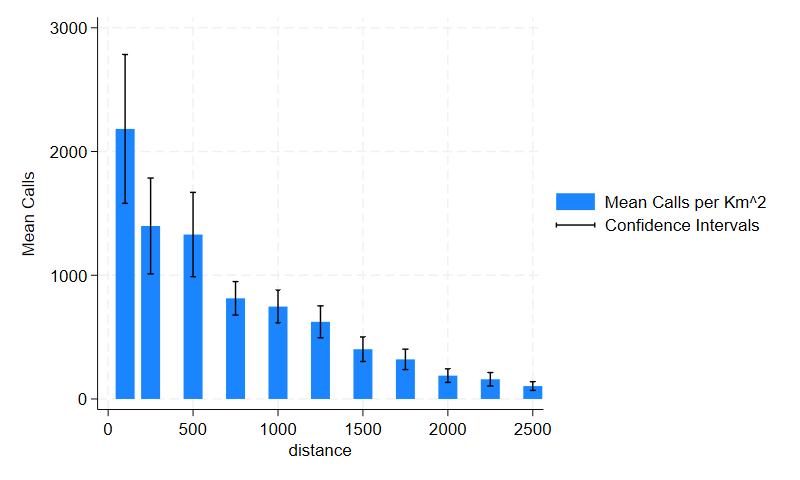
\includegraphics[width=0.75\linewidth]{Reproducibility Package/Visual Graphics/Crime_CI_Graph.png}
    \caption{Mean Crime Calls per SATC per distance group}
    \label{fig:Figure4}
        \textit{X-axis consist of the different distance groups used. Distance measured in meters.}
    \textit{Y-axis is measured in mean calls per kilometers squared.}
     \textit{Confidence thresholds measured at 90\%.}
\end{figure}

Figure~\ref{fig:Figure3} represents the mean calls per SATC per kilometer squared by distance group in a bar graph. These are the average calls for the total 911 call set per SATC. Figure~\ref{fig:Figure3} uses the same data as Table~\ref{tabl:Table1} and represents the same means and significance levels. Figure~\ref{fig:Figure4} represents the mean crime-related calls per SATC per square kilometer by distance groups in a bar graph. Figure~\ref{fig:Figure4} uses the same data as Table~\ref{tabl:Table2} and represents the same means and significance levels used. The confidence level of 90\% for mean calls is overlaid on top of their respective distance groups. 

The confidence intervals of 250-500 meters and 750-1000 meters significantly overlap, as the confidence interval of the larger distance group overlaps the mean and the confidence interval of the smaller distance group. This is true for both Figure~\ref{fig:Figure3} and Figure~\ref{fig:Figure4}. This indicates that there is no statistical significance in the difference between the means of these two groups, which is supported by the p-values found in Table~\ref{tabl:Table1} and Table~\ref{tabl:Table2}. This large overlap means that there is no correlation between the mean 911 calls per SATC and their distance group. 

The other confidence intervals do have some overlap with the sequential intervals, but not as much. These confidence intervals in Figure~\ref{fig:Figure3} include 100-250 meters, 500-750 meters, 1000-1250 meters, 1250-1500 meters, 1500-1750 meters, 1750-2000 meters, 2000-2250 meters, and 2250-2750 meters. Due to the size of the graph, the last three confidence intervals are hard to visually identify, so looking at the p-values is crucial. Figure~\ref{fig:Figure4} also follows these same trends. The only difference is that the y-axis is smaller since there are fewer observations in total. Within these distance group pairs, the larger distance group interval does not extend past the mean of the smaller distance group. This means that 90\% of the time, the larger distance group's mean will not be the same as the smaller distance group's mean calls. This suggests a small statistical significance. These observations additionally support the p-values observed in Table~\ref{tabl:Table1} and Table~\ref{tabl:Table2}, as the p-values for these distance group pairs are statistically significant within the 0.10 significance level. 


%Explain what analyses you did, provide evidence (like in the descriptive stats exercise, but refined and clear) and then explain what your results mean.
\break
\section{Discussion}
\label{sec:discussion}

One theory on why we find that as distance from a treatment center increases, the rate of 911 calls decreases is due to the positive feedback loop between drugs, crime, and lower standards of living in the area. SATCs are more likely to be built in areas where drug use is prevalent, since higher levels of drug use are associated with a lower standard of living in an area. (\cite{drugs_and_crime}). This creates a positive feedback loop between increased drug use and lower living standards, leading to the establishment of SATCs. Moreover, \cite{drugs_and_crime} shows that lower standards of living are linked to higher crime rates and, consequently, reduced safety in an area. Therefore, SATCs in areas where drug usage is prevalent decrease the living standard, thereby reducing safety and increasing crime. The lack of safety, in turn, leads to more 911 calls.  

Additionally, Detroit may have placed SATCs in neighborhoods with lower living standards due to pressure from more affluent communities. More affluent communities tend to exhibit a "Not In My Backyard" (NIMBY) mentality, opposing the placement of SATCs in their neighborhoods (\cite{NIMBY}). This resistance stems from the fear or stigma residents have about drug users. They might perceive SATCs as bringing dangerous or mentally ill people into their area, impacting the safety of the area. Thus, higher standard-of-living neighborhoods tend to lobby for NIMBY policies in their communities, pushing SATC to be in areas that do not have the resources to oppose their placement.

Furthermore, higher standard-of-living areas tend to have lower crime rates in general. High standards of living decrease crime, which creates a positive feedback system in these neighborhoods, potentially explaining why the farther a ring is from a SATC, the fewer 911 calls there are on average. Therefore, the distance rings that have fewer 911 calls on average could be on the cusp of, or geographically in neighborhoods that do not have SATCs. 
    
Another explanation for the lower frequency of 911 calls in further distance rings could be that we only consider each 911 call once in our analysis. When we geo-code the 911 calls, we assign each observation to only one SATC, the one geographically closest to it. The methodology behind this is to limit any overlap between 911 calls due to SATCs being geographically close together. Without this step, it could exaggerate the frequencies of 911 calls relative to an SATC and effect our measures in the smaller distance rings.  However, in farther distance rings, a call might be similar in distance to two SATCs but will only be assigned to one, when in reality, it could be assigned to either SATC. This could possibly lead to an underrepresentation of the frequency of 911 calls in the further distance rings. Therefore, this process of analysis could potentially be improved upon through finding a valid statistical test that would allow us to double count 911 calls, which could help resolve this issue. 

Moreover, one significant limitation was the inability to fine-tune 911 call data to determine whether calls were directly related to drug activity. Without additional data, such as toxicology reports or detailed incident descriptions, it remains challenging to assess the role of drugs in criminal behavior or whether the crimes involved were violent. A better understanding of what calls were drug-related or induced could provide more accurate results on the relationship between drug abuse, crime, and the role of a SATC in amplifying or mitigating crime in an area. 
    
Another limitation is the population density of this urban sample. The observed pattern of 911 calls can be influenced by higher population density in more urban parts of Detroit. An increasing population in these areas naturally increases the number of emergency calls. However, specific information on the population density of a small geographical area, such as a city block, is not publicly available. Therefore, in in order to accurately consider population density in relation to the number of 911 calls we would need to geographically expand our area of analysis. However, expanding the geographical unit of analysis would not accurately allow us to study the effects an SATC has on the community immediately surrounding it. 

Our group analyzes data only from the year 2017. However, considering more years in our analysis would likely give us more statistical power. Therefore, we see future research supporting these findings or a stronger pattern through two possible ways. Firstly, by utilizing cross-sectional data for more than one year which would likely strengthen the correlational relationships we found in this paper. Secondly, by analyzing time series data based on the openings and closings of SATCs. This option could identify a causal impact of the presence of a SATC in a neighborhood regarding 911 calls and, consequentially, crime rates. These results could impact policymaking decisions regarding where to fund and support the placement of SATC to serve populations in need. 

\section{Conclusion}
\label{sec:conclusion}

We hypothesized that as the distance from a SATC increases, the frequency of 911 calls also increases. The closer a SATC is, the more accessible it is. A closer treatment center should reduce crime rates in the area, as measured by 911 calls. We conducted a cross-sectional analysis to examine how the distance from an SATC affects the frequency of 911 calls. Our results show that contrary to our hypothesis, as distance from a SATC increases, the amount of 911 calls per square kilometer decreases. This distance decay relationship indicates a relationship between SATC placements and 911 calls but in the opposite direction of the original hypothesis. We theorize that this could be due to the Not In My Backyard movement to prevent SATCs in areas with a higher standard of living, the way we geo-coded our data to only count every 911 call once, or our use of 911 calls as proxy data for crime. 



 
%Re-state (in different words) what you did and what you learned. If your discussion (Section 6) would be short, you can just have a Conclusion section that includes your discussion (that is, leave out a separate Discussion section).

\newpage
\singlespacing
\setlength\bibsep{0pt}
\bibliography{WorkingFolder/sources}
\bibliographystyle{chicago}



\newpage
\section*{Data Appendix} \label{sec:appendixa}
\addcontentsline{toc}{section}{Appendix A}

Our replication package:

\href{https://github.com/ecn310/course-project-zipcentercrime/tree/main/Reproducibility%20Package}{https://github.com/ecn310/course-project-zipcentercrime/tree/main/Reproducibility\%20Package}

\vspace{10pt}

% essentially, we should have a bunch of links to our files in the appendix section. 

The data files, code, and documentation for this project are found in the zipcentercrime \href{https://github.com/ecn310/course-project-zipcentercrime}{GitHub Repository}. All information and files necessary to reproduce these results can be accessed by this the \href{https://github.com/ecn310/course-project-zipcentercrime/tree/main/Reproducibility%20Package}{reproducibility package}. Access to the code can be found in the \href{https://github.com/ecn310/course-project-zipcentercrime/tree/main/Reproducibility%20Package/Do%20files}{Do Files Folder}, and access the figures from this folder \href{https://github.com/ecn310/course-project-zipcentercrime/tree/main/Reproducibility%20Package/Visual%20Graphics}{visual folder here}. 

Use Stata 18.0 to isolate data to the year 2017 and the final data analysis. Use ArcGIS Pro to geo-code the call points and SATC points. 

The original 911 calls dataset can be accessed from the \href{https://data.detroitmi.gov}{The City of Detroit Open Data Portal}. The raw dataset can be accessed from zipcentercrime repository from the \href{https://github.com/ecn310/course-project-zipcentercrime/blob/main/Reproducibility%20Package/RawData/Acess_calls_final_data_set.md}{Acess\_calls\_final\_data\_set.md}. The original SATC dataset can be accessed from the \href{https://www.samhsa.gov}{SAMHSA website}. The raw dataset can be downloaded from the zipcentercrime repository through the \href{https://github.com/ecn310/course-project-zipcentercrime/blob/main/Reproducibility%20Package/RawData/detroit_samhsa_sud_2015_2021.dta}{detroit\_samhsa\_sud\_2015\_2021.dta file}.

% Above is the skeleton version of the new data appendix. It is based on Ryan's data appendix. If someone can add links to the parenthesis that would be great. We also need to clean up any files that we aren't using in the final dataset, but that should be the last thing we do before we submit. 


% \begin{table}[h]
%\centering
%\caption{Ratio Analysis}
%begin{tabular}{l||c|c|cc|c|c}
%\hline\hline
 %           &ratio\_results&            &            &            &            &            \\
     %       &       Ratio&   Std. Err.&  [95 5Conf.&   Interval]&     T score&     P value\\
%\hline
%100/250     &    1.518016&     .305492&     .901933&      2.1341&    4.969087&    .0000112\\
%250/500     &    1.112848&    .1703623&    .7692794&    1.456416&    6.532241&    6.14e-08\\
%500/750     &    1.571244&    .1966827&    1.174596&    1.967893&    7.988725&    4.92e-10\\
%750/1000    &    1.091451&    .1104992&    .8686081&    1.314294&    9.877456&    1.25e-12\\
%1000/1250   &    1.189354&    .0748615&    1.038382&    1.340327&     15.8874&    1.32e-19\\
%1250/1500   &    1.461179&    .1268808&    1.205299&    1.717058&    11.51615&    1.00e-14\\
%1500/1750   &    1.365242&    .1935897&    .9748308&    1.755652&    7.052244&    1.08e-08\\
%1750/2000   &     1.66361&    .2204068&    1.219117&    2.108103&    7.547907&    2.09e-09\\
%2000/2250   &    1.204906&     .110774&    .9815093&    1.428303&    10.87716&    6.33e-14\\
%2250/2500   &    1.519659&    .1688579&    1.179124&    1.860193&     8.99963&    1.91e-11\\
%\hline\hline
%\end{tabular}
%\flushleft
%\begin{footnotesize}
%\begin{singlespace}
%\textbf{Note 1}: A larger T score indicates the estimated coefficient is more significantly different from the hypothesized value.
%\textbf{Note 2}: A smaller P value p<0.05 means the result is statistically significant. This means the estimated coefficient is likely not zero.
%\end{singlespace}
%\end{footnotesize}
%\end{table} %

\end{document}